\documentclass[a4paper, 11pt]{article}

\usepackage[utf8]{inputenc}
\usepackage[czech]{babel}
\usepackage[left=2cm, text={17cm, 24cm}, top=3cm]{geometry}
\usepackage{times}	% Times New Roman font
\usepackage{pdflscape}
\usepackage{multirow}
\usepackage[ruled]{algorithm2e}
\usepackage{algorithmic}
\usepackage{graphicx}
\usepackage{picture}

\graphicspath{ {./include/} }

%\floatname{algorithm2e}{Algoritmus}
\renewcommand{\algorithmcfname}{Algoritmus}
\renewcommand{\algorithmicrequire}{\textbf{Input:}}
\renewcommand{\algorithmicensure}{\textbf{Output:}}

\begin{document}

\begin{titlepage}

\begin{center}

\textsc{{\Huge Vysoké učení technické v~Brně}\\\medskip{\huge Fakulta informačních technologií}}

\vspace{\stretch{0.382}}

{\LARGE Typografie a publikování -- 3. projekt}\\\medskip{\Huge Tabulky a obrázky}

\vspace{\stretch{0.618}}

%\enlargethispage{0.5cm}

{\Large 28. března 2017 \hfill Jakub Frýz}

\end{center}

\end{titlepage}

\section{Úvodní strana}

Název práce umístěte do~zlatého řezu a~nezapomeňte uvést dnešní datum a~vaše jméno a~příjmení.

\section{Tabulky}

Pro sázení tabulek můžeme použít buď prostředí\ \ \texttt{tabbing}\ \ nebo prostředí\ \ \texttt{tabular}.

\subsection{Prostředí\ \ \texttt{tabbing}}

Při použití\ \ \texttt{tabbing}\ \ vypadá tabulka následovně:

\begin{tabbing}
Vodní Melouny\quad	\= 25,90\quad	\= Množství	\kill
\textbf{Ovoce}	\> \textbf{Cena	}	\> \textbf{Množství}	\\
Jablka			\> 25,90			\> 3 kg					\\
Hrušky			\> 27,40			\> 2,5 kg				\\
Vodní Melouny	\> 35,--			\> 1 kus				\\
\end{tabbing}

\noindent Toto prostředí se dá také použít pro sázení algoritmů, ovšem vhodnější je použít prostředí\ \ \texttt{algorithm}\ \ nebo\ \ \texttt{algorithm2e}\ \ (viz sekce \ref{algoritmy}).

\subsection{Prostředí\ \ \texttt{tabular}}

Další možností, jak vytvořit tabulku, je použít prostředí\ \ \texttt{tabular}. Tabulky pak budou vypadat takto\footnote{Kdyby byl problem s \texttt{cline}, zkuste se podívat třeba sem: http://www.abclinuxu.cz/tex/poradna/show/325037}:

\begin{table}[h]
\catcode`\-=12
\centering
\begin{tabular}{|l|r|r|}
\hline
\multicolumn{1}{|c|}{\textbf{}} & \multicolumn{2}{c|}{\textbf{Cena}} \\ \cline{2-3} 
\textbf{Měna} & \multicolumn{1}{c|}{\textbf{nákup}} & \multicolumn{1}{c|}{\textbf{prodej}} \\ \hline
EUR & 27,02 & 27,20 \\ \hline
GBP & 31,08 & 31,80 \\ \hline
USD & 25,15 & 25,51 \\ \hline
\end{tabular}
\caption{Tabulka kurzů k dnešnímu dni}
\label{kurzy}
\end{table}

\begin{table}[h]
\catcode`\-=12
\centering

\begin{tabular}{cccc}

\begin{tabular}{|l|l|}
\hline
$A$ & $\neg A$ \\ \hline
\textbf{P} & N \\ \hline
\textbf{O} & O \\ \hline
\textbf{X} & X \\ \hline
\textbf{N} & P \\ \hline
\end{tabular}

\begin{tabular}{|c|c|c|c|c|c|}
\hline
\multicolumn{2}{|c|}{\multirow{2}{*}{$A \land B$}} & \multicolumn{4}{c|}{$B$} \\ \cline{3-6} 
\multicolumn{2}{|c|}{} & \textbf{P} & \textbf{O} & \textbf{X} & \textbf{N} \\ \hline
\multirow{4}{*}{$A$} & \textbf{P} & P & O & X & N \\ \cline{2-6} 
 & \textbf{O} & O & O & N & N \\ \cline{2-6} 
 & \textbf{X} & X & N & X & N \\ \cline{2-6} 
 & \textbf{N} & N & N & N & N \\ \hline
\end{tabular}

\begin{tabular}{|c|c|c|c|c|c|}
\hline
\multicolumn{2}{|c|}{\multirow{2}{*}{$A \lor B$}} & \multicolumn{4}{c|}{$B$} \\ \cline{3-6} 
\multicolumn{2}{|c|}{} & \textbf{P} & \textbf{O} & \textbf{X} & \textbf{N} \\ \hline
\multirow{4}{*}{$A$} & \textbf{P} & P & P & P & P \\ \cline{2-6} 
 & \textbf{O} & P & O & P & O \\ \cline{2-6} 
 & \textbf{X} & P & P & X & X \\ \cline{2-6} 
 & \textbf{N} & P & O & X & N \\ \hline
\end{tabular}

\begin{tabular}{|c|c|c|c|c|c|}
\hline
\multicolumn{2}{|c|}{\multirow{2}{*}{$A \to B$}} & \multicolumn{4}{c|}{$B$} \\ \cline{3-6} 
\multicolumn{2}{|c|}{} & \textbf{P} & \textbf{O} & \textbf{X} & \textbf{N} \\ \hline
\multirow{4}{*}{$A$} & \textbf{P} & P & O & X & N \\ \cline{2-6} 
 & \textbf{O} & P & O & P & O \\ \cline{2-6} 
 & \textbf{X} & P & P & X & X \\ \cline{2-6} 
 & \textbf{N} & P & P & P & P \\ \hline
\end{tabular}

\end{tabular}

\caption{Protože Kleeneho trojhodnotová logika už je \uv{zastaralá}, uvádíme si zde příklad čtyřhodnotové logiky}
\label{logika}
\end{table}

\pagebreak

\section{Algoritmy}\label{algoritmy}

Pokud budeme chtít vysázet algoritmus, můžeme použít prostředí\ \ \texttt{algorithm}\footnote{Pro nápovědu, jak zacházet s prostředím \texttt{algorithm}, můžeme zkusit tuhle stránku:\\ http://ftp.cstug.cz/pub/tex/CTAN/macros/latex/contrib/algorithms/algorithms.pdf.}\ \ nebo\ \ \texttt{algorithm2e}\footnote{Pro \texttt{algorithm2e} zase tuhle: http://ftp.cstug.cz/pub/tex/CTAN/macros/latex/contrib/algorithm2e/algorithm2e.pdf.}. Příklad použití prostředí\ \ \texttt{algorithm2e}\ \ viz Algoritmus \ref{fastslam}.

\medskip

\begin{algorithm}
\caption{\textsc{FastSLAM}}
\label{fastslam}
\begin{algorithmic}[1]
	\REQUIRE $(X_{t-1}, u_t, z_t)$
	\ENSURE $X_t$
	\STATE $\overline{X_t} = X_t = 0$
	\FOR{$k = 1$ to $M$}
		\STATE $x_t^{[k]} = \mbox{\textit{sample\_motion\_model}}(u_t, x_{t-1}^{[k]})$
		\STATE $\omega_t^{[k]} = \mbox{\textit{measurement\_model}}(z_t, x_t^{[k]}, m_{t-1})$
		\STATE $m_t^{[k]} = updated\_occupancy\_grid(z_t, x_t^{[k]}, m_{t-1}^{[k]})$
		\STATE $\overline{X_t} = \overline{X_t} + \langle x_x^{[m]}, \omega_t^{[m]} \rangle$
	\ENDFOR
	\FOR{$k = 1$ to $M$}
		\STATE draw $i$ with probability $\approx \omega_t^{[i]}$
		\STATE add $\langle x_x^{[k]}, m_t^{[k]} \rangle$
	\ENDFOR
	\RETURN $X_t$
\end{algorithmic}
\end{algorithm}

\section{Obrázky}

Do našich článků můžeme samozřejmě vkládat obrázky. Pokud je obrázkem fotografie, můžeme klidně použít bitmapový soubor. Pokud by to ale mělo být nějaké schéma nebo něco podobného, je dobrým zvykem takovýto obrázek vytvořit vektorově.

\begin{figure}[h]
\centering
\scalebox{0.40}{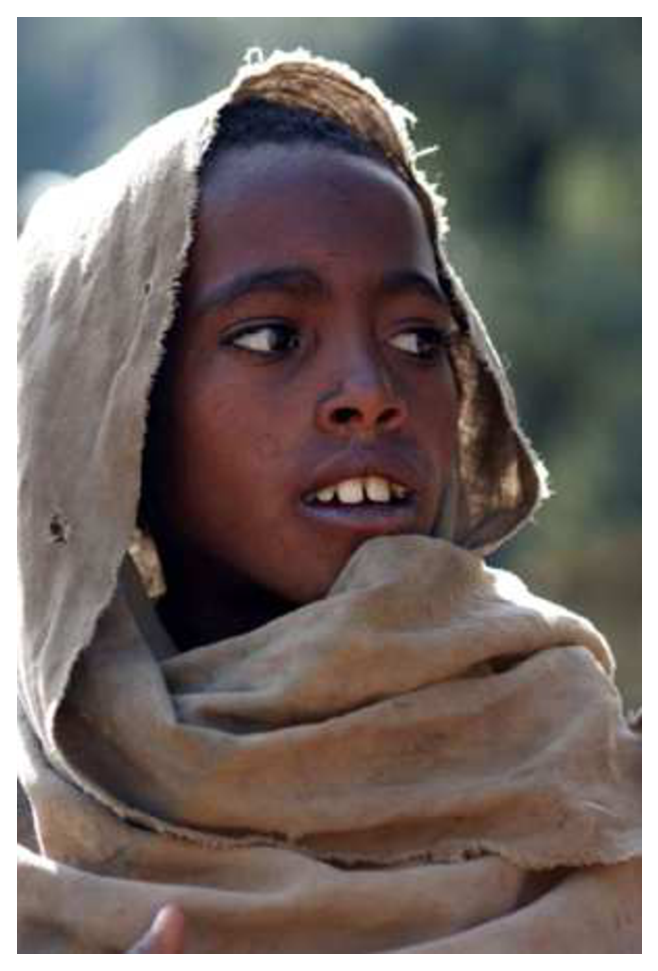
\includegraphics{etiopan.eps}\reflectbox{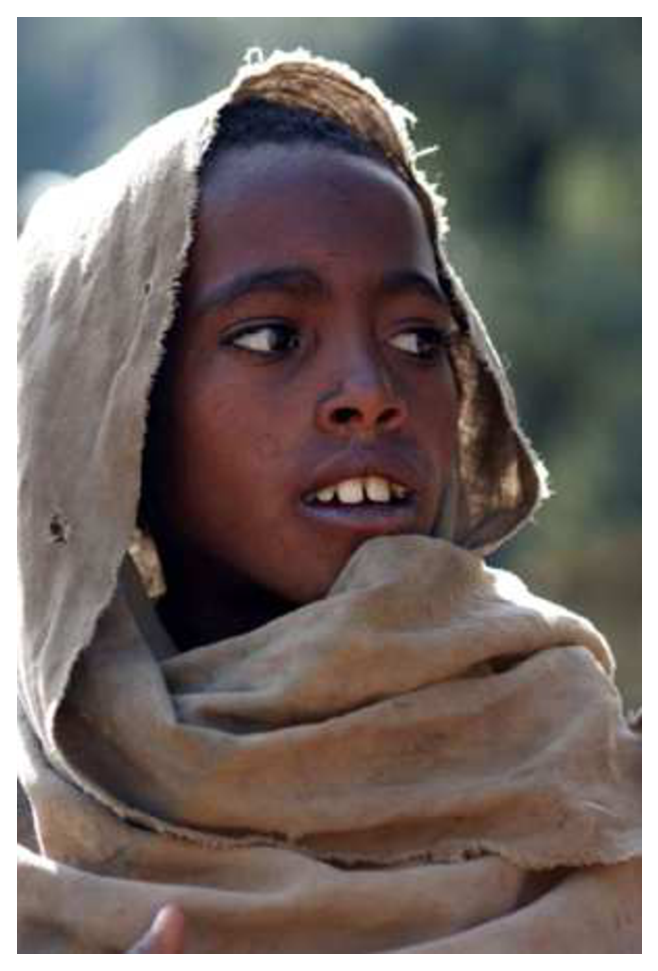
\includegraphics{etiopan.eps}}}
\caption{Malý Etiopánek a jeho bratříček}
\label{etiop}
\end{figure}

\pagebreak

Rozdíl mezi vektorovým\ldots

\begin{figure}[h]
\centering

\includegraphics[width=0.50\textwidth]{oniisan.eps}
\caption{Vektorový obrázek}
\label{vektor}
\end{figure}

\noindent\ldots a bitmapovým obrázkem

\begin{figure}[h]
\centering

\includegraphics[width=0.55\textwidth]{oniisan2.eps}
\caption{Vektorový obrázek}
\label{rastr}
\end{figure}

\noindent se projeví například při zvetšení.

Odkazy (nejen ty) na obrázky \ref{etiop}, \ref{vektor} a \ref{rastr}, na tabulky \ref{kurzy} a \ref{logika} a také na algoritmus \ref{fastslam} jsou udělány pomocí 
křížových odkazů. Pak je ovšem potřeba zdrojový soubor přeložit dvakrát. 

Vektorové obrázky lze vytvořit i přímo v \LaTeX u, například pomocí prostředí\ \ \texttt{picture}.

\pagebreak

\begin{landscape}

\begin{figure}[t]
\begin{picture}(500,100)
	\linethickness{0.75mm}
	\put(50,0){\framebox(600,250)}
	\linethickness{1.5mm}
	\put(60,25){\line(1,0){580}}
	\linethickness{0.25mm}
	\put(100,25){\line(0,1){125}}
	\put(140,25){\line(0,1){50}}
	\put(140,75){\line(1,0){110}}
	\put(250,75){\line(5,-2){125}}
	\put(100,150){\line(1,0){150}}
	\put(250,125){\line(0,1){50}}
	\put(250,175){\line(1,0){200}}
	\put(450,175){\line(0,-1){50}}
	\put(175,125){\line(1,0){400}}
	\put(175,105){\line(1,0){400}}
	\put(175,105){\line(0,1){20}}
	\put(575,105){\line(0,1){20}}
	\put(175,105){\line(6,-5){37}}
	\put(450,135){\line(1,0){115}}
	\put(565,135){\line(0,-1){10}}
	\put(290,60){\line(1,0){285}}
	\put(575,60){\line(0,-1){35}}
	\put(270,65){\line(0,1){35}}
	\put(270,100){\line(1,0){290}}
	\put(560,100){\line(0,-1){40}}
	\put(550,200){\circle{60}}
\end{picture}
\caption{Vektorový obrázek}
\end{figure}

\end{landscape}


\end{document}
